\documentclass[tikz,border=2pt]{standalone}
\usepackage{amsmath}
\usepackage{pgfplots}
\usepgfplotslibrary{groupplots}
\pgfplotsset{compat=1.18}
\definecolor{trivial}{RGB}{166,213,226}
\definecolor{tsc}{RGB}{180,159,205}
\definecolor{boundary}{RGB}{74,58,126}
\definecolor{nuone}{RGB}{220,139,142}
\definecolor{tscminus}{RGB}{228,200,145}
\definecolor{profilea}{RGB}{0,87,184}
\definecolor{profileb}{RGB}{198,40,40}
\definecolor{profilemid}{RGB}{0,0,0}
\begin{document}
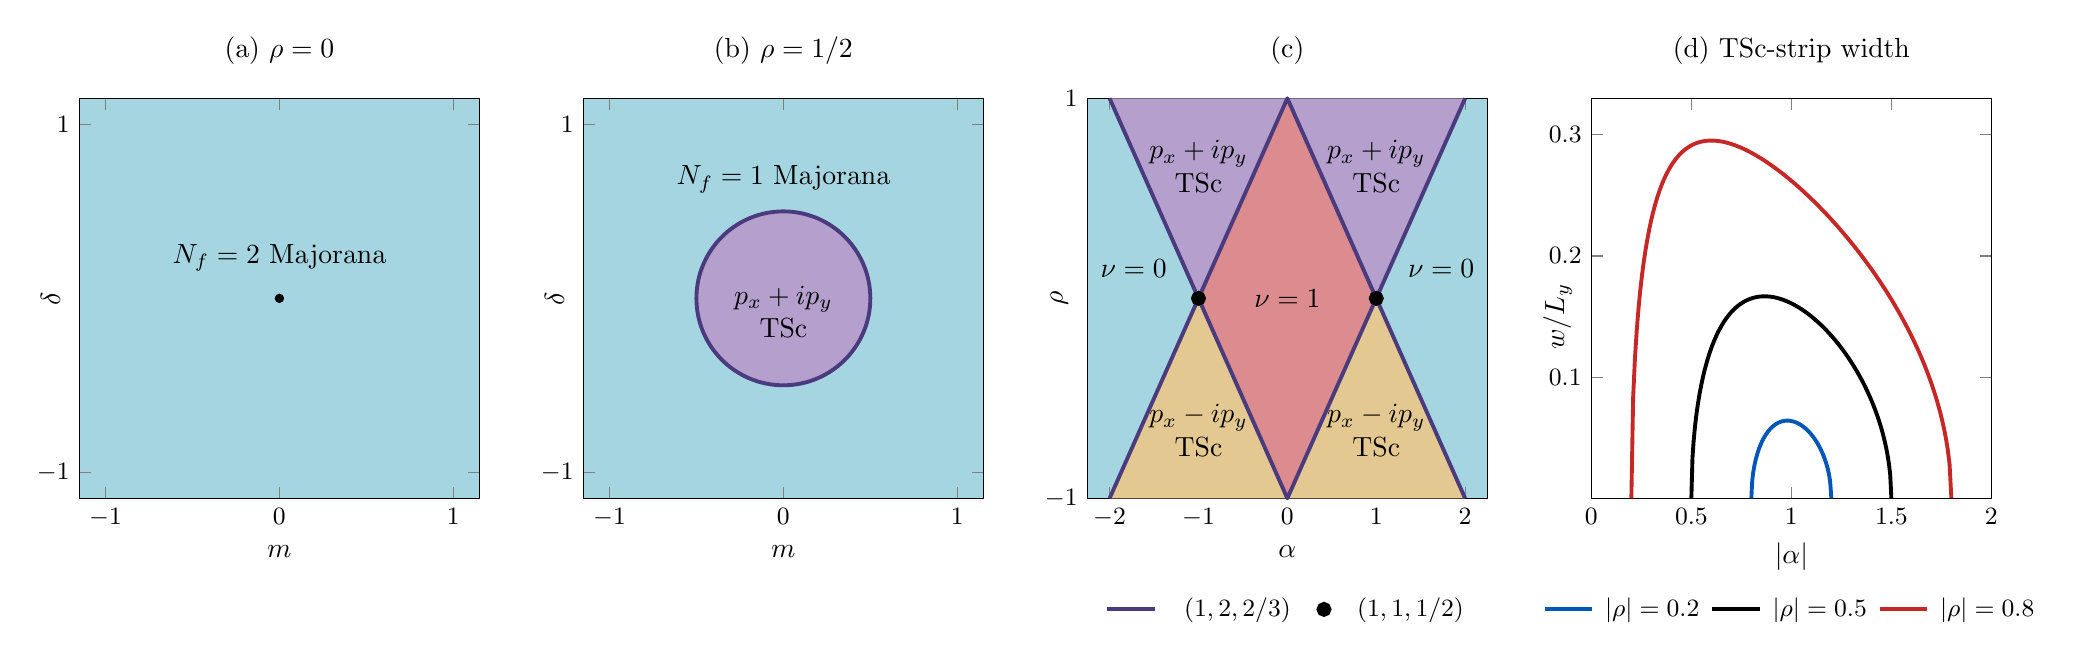
\begin{tikzpicture}
\begin{groupplot}[
 group style={group size=4 by 1,horizontal sep=.52in},
 scale only axis,width=2in,height=2in,
 clip=false,
 axis line style={line width=.55pt},tick style={line width=.45pt},
 label style={font=\normalsize},tick label style={font=\small},
 ylabel style={at={(axis description cs:-.04,.5)},anchor=south,inner sep=1pt},
 every node/.append style={font=\normalsize},
 every axis plot/.append style={line width=1.4pt}]
\nextgroupplot[
 axis equal image,xmin=-1.15,xmax=1.15,ymin=-1.15,ymax=1.15,
 xtick={-1,0,1},ytick={-1,1},xlabel={$m$},ylabel={$\delta$},
 axis background/.style={fill=trivial}]
\fill[black] (axis cs:0,0) circle[radius=.027];
\node[anchor=south] at (axis cs:0,.10) {$N_f=2$ Majorana};
\node[anchor=south] at (rel axis cs:.5,1.06) {(a) $\rho=0$};

\nextgroupplot[
 axis equal image,xmin=-1.15,xmax=1.15,ymin=-1.15,ymax=1.15,
 xtick={-1,0,1},ytick={-1,1},xlabel={$m$},ylabel={$\delta$},
 axis background/.style={fill=trivial}]
\fill[tsc,draw=boundary,line width=1.4pt] (axis cs:0,0) circle[radius=.5];
\node[align=center] at (axis cs:0,-.08) {$p_x+i p_y$\\TSc};
\node[anchor=south] at (axis cs:0,.55) {$N_f=1$ Majorana};
\node[anchor=south] at (rel axis cs:.5,1.06) {(b) $\rho=1/2$};

\nextgroupplot[
 xmin=-2.25,xmax=2.25,ymin=-1,ymax=1,
 xtick={-2,-1,0,1,2},ytick={-1,1},
 xlabel={$\alpha$},ylabel={$\rho$},
 axis background/.style={fill=trivial},
 legend columns=2,
 legend style={draw=none,at={(.5,-.22)},anchor=north,
               font=\small,column sep=8pt}]
\fill[nuone] (axis cs:-1,0)--(axis cs:0,1)
 --(axis cs:1,0)--(axis cs:0,-1)--cycle;
\pgfplotsinvokeforeach{-1,1}{
 \fill[tsc] (axis cs:#1,0)--(axis cs:{#1-1},1)
  --(axis cs:{#1+1},1)--cycle;
 \fill[tscminus] (axis cs:#1,0)--(axis cs:{#1-1},-1)
  --(axis cs:{#1+1},-1)--cycle;
 \node[align=center] at (axis cs:#1,.66) {$p_x+i p_y$\\TSc};
 \node[align=center] at (axis cs:#1,-.66) {$p_x-i p_y$\\TSc};
}
\draw[boundary,line width=1.4pt,line join=round]
 (axis cs:-2,1)--(axis cs:-1,0)--(axis cs:0,1)
 --(axis cs:1,0)--(axis cs:2,1)
 (axis cs:-2,-1)--(axis cs:-1,0)--(axis cs:0,-1)
 --(axis cs:1,0)--(axis cs:2,-1);
\node at (axis cs:0,0) {$\nu=1$};
\node at (axis cs:-1.73,.15) {$\nu=0$};
\node at (axis cs:1.73,.15) {$\nu=0$};
\addlegendimage{boundary,line width=1.4pt}
\addlegendentry{$(1,2,2/3)$}
\addplot[only marks,mark=*,mark size=2pt,black]
 coordinates {(-1,0) (1,0)};
\addlegendentry{$(1,1,1/2)$}
\node[anchor=south] at (rel axis cs:.5,1.06) {(c)};

\nextgroupplot[
 xmin=0,xmax=2,ymin=0,ymax=.33,
 xtick={0,.5,1,1.5,2},ytick={.1,.2,.3},
 ylabel style={at={(axis description cs:-.04,.455)},anchor=south,inner sep=1pt},
 xlabel={$|\alpha|$},ylabel={$w/L_y$},
 legend columns=3,
 legend style={draw=none,at={(.5,-.22)},anchor=north,
               font=\small,column sep=2pt}]
\addplot[profilea,domain=.8:1.2,samples=180]
 {acos(min(1,max(-1,(1+x^2-.2^2)/(2*x))))/180};
\addlegendentry{$|\rho|=0.2$}
\addplot[profilemid,domain=.5:1.5,samples=180]
 {acos(min(1,max(-1,(1+x^2-.5^2)/(2*x))))/180};
\addlegendentry{$|\rho|=0.5$}
\addplot[profileb,domain=.2:1.8,samples=180]
 {acos(min(1,max(-1,(1+x^2-.8^2)/(2*x))))/180};
\addlegendentry{$|\rho|=0.8$}
\node[anchor=south] at (rel axis cs:.5,1.06) {(d) TSc-strip width};
\end{groupplot}
\end{tikzpicture}
\end{document}
